%%%%%%%%%%%%%%%%%%%%%%%%%%%%%%%%%%%
%                 Wrocław, październik 2012r.
%    Pracownia z Analizy Numerycznej M
%      Sprawozdanie z zadania p1.11
%         Łukasz Czapliński
%%%%%%%%%%%%%%%%%%%%%%%%%%%%%%%%%%%
\documentclass[11pt,wide]{mwart}

\usepackage[utf8]{inputenc} 
\usepackage[OT4,plmath]{polski}
\usepackage{graphicx}      
\usepackage{caption}
\usepackage{subcaption}
\usepackage{longtable}
\usepackage{amsmath,amssymb,amsfonts,amsthm,mathtools}
                            
\usepackage{bbm}           
\usepackage[colorlinks=true]{hyperref}
                          
\usepackage{url}
%%%%%%%%%%%%%%%%%%%%%%%%%%%%%%%%%5
\title{{\textbf{Pracownia z analizy numerycznej\\}}
       {\Large Sprawozdanie do zadania \textbf{P1.11}\\}
       {\large Prowadzący: dr Paweł Woźny}}
\author{Łukasz Czapliński\\  e-mail: \texttt{czapl.luk@gmail.com}}
\date{Wrocław, dnia \today\ r.}

\begin{document}
\thispagestyle{empty}
\maketitle
\newpage
\section{Wstęp}
\subsection{Oznaczenia}
\begin{table}[h]
    \centering
    \begin{tabular}{l l}
        \hline
        $\Phi(n)$ & przybliżenie $e^n$ liczone z szeregu Taylora bez przekształceń\\
         $\Psi(n)$ & przybliżenie $e^n$ liczone z użyciem funkcji $\Phi$ i pewnego usprawnienia\\
        $exp(n)$  & funkcja wbudowana licząca $e^n$ (z biblioteki dla C++ $<cmath>$)\\
        $T(f,n)$  & czas liczenia funkcji $f$ dla argumentu $n$\\
        \hline
    \end{tabular}
    \caption{Użyte oznaczenia}
    \label{tab:oznaczenia}
\end{table}
\subsection{Omówienie problemu}
Funkcja $e^x$ pojawia się w problemach numerycznych niezwykle często. Jej obliczanie z dobrą dokładnością nie jest tak trywialne jak liczenie wartości funkcji wykładniczej, której podstawa jest wymierna. Celem tej pracy będzie porównanie kilku sposobów obliczania tej funkcji, ich dokładności i czasu działania.
\subsubsection{Uwarunkowanie zadania}
Uwarunkowanie zadania obliczania funkcji jednej zmiennej $f$, która w dodatku jest ciągła i ma pochodna, można obliczyć wzorem: \\
\begin{gather}
    C(f,x) = |\frac{x*f'(x)} { f(x)}|\\
    C(e^x, x) = |\frac{x*(e^x)'}{ e^x}| = |x|
\end{gather}\\
Jak widać, w przypadku obliczania funkcji $e^x$ oznacza to, ze błąd względny jest liniowo zależny od argumentu. Oznacza to, ze obarczone błędem uwarunkowania (czyli efektem zwielokrotnienia małego początkowego zaburzenia danych) może być tylko liczenie wartości funkcji dla bardzo dużych (co do wartości bezwzględnej) argumentów.
\subsection{Uzyte metody}
Pierwsza z użytych metod, $\Phi(x)$, liczy wartość $e^x$ ze wzoru
\begin{math}
    e^x = \sum_{i=1}^{\infty}\frac{x^i}{i!}
\end{math}
. \\
\indent
Druga metoda, $\Psi(x)$, wykorzystuje fakt, iż $e^x = 2^m*e^u$, gdzie $m\in \mathbb{Z}$, a $|u| < \frac{\ln 2}{2}$. Uzasadnienie tego faktu znajduje się w kolejnej sekcji. Sprowadza to liczenie $e^x$ do liczenia $e^u$, ponieważ $2^m$ może być policzone jedna komenda procesora (zakładając, że wartość ta mieści się w naszej arytmetyce). Dodatkowo, szereg Maclaurina dla funkcji $e^x$ dla argumentów bliskich zera jest bardzo szybko zbieżny.
\subsubsection{Wzory matematyczne i ich wyprowadzenia}
Wzór, z którego korzysta pierwsza metoda, to oczywiście rozwinięcie funkcji $e^x$ w szereg Maclaurina:\\
\begin{gather}
        f(x) = \sum_{i=0}^{\infty}\frac{f^{(i)}(0)*x^i}{i!}\\
        (e^x)' = e^x\\
            e^0 = 1
\end{gather}
\\stąd: \\
\begin{gather}
        e^x = \sum_{i=0}^{\infty}\frac{x^i}{i!}
\end{gather}
\\
\indent Z kolei uzasadnieniem drugiej metody jest fakt:\\
\begin{gather}
    \forall x\in \mathbb{R} : \exists m\in \mathbb{Z}, u\in \mathbb{R} :
    |u| < \frac{\ln 2}{2} \wedge x = m*\ln 2 + u
\end{gather}
\\z którego wynika: \\
\begin{gather}
          e^x = e^{(m*\ln 2 + u)}\\
    e^{(m*\ln 2 + u)} = e^{(m*\ln 2)} * e^u\\
    e^{(m*\ln 2)} = 2^m
\end{gather}
\\ stąd: \\
\begin{gather}
        e^x = 2^m*e^u
\end{gather}
\subsubsection{O programie}
Użyty do doświadczenia (i załączony) program napisany jest w C++ i używa arytmetyki typu double (64 bitowa). Zaimplementowane w nim są obie metody: $\Phi(x)$, $\Psi(x)$. \\
\indent Metoda $\Phi$ używa akumulatora, by sumować wartości $\frac{x^i}{i!}$ dla kolejnych $i$ tak długo, dopóki oczekiwany błąd nie przekroczy danej granicy (użyto wartości $\epsilon = 10^{-12}$). Warto zauważyć, ze wartość $\frac{x^i}{i!}$ nie jest liczona w każdej iteracji, lecz używana jest wartość z poprzedniej iteracji wedle wzoru: \\
\begin{gather}
        it(i, x) = \frac{x^i}{i!}\\
        it(1, x) = x\\
                it(i+1, x) = (it(i, x)/(i+1))*x
\label{eq:phiblad}
\end{gather}

\indent Z kolei metoda $\Psi$ najpierw oblicza $m$ i $u$, a następnie wywołuje metodę $\Phi(u)$. Uzyskany wynik jest równy \\
\begin{gather}
        \Psi(m*\ln 2 + u) = 2^m * \Phi(u)
\label{eq:psiblad}
\end{gather}
\indent Sam program jest poniekąd interaktywny: po włączeniu oczekuje na jedno z poleceń: "s", "m", "b" lub "e". Po otrzymaniu odpowiedniego polecenia wypisuje na standardowe wyjście wyniki obliczeń funkcji $\Phi$, $\Psi$ i $exp$ dla argumentów z przedziału (odpowiednio dla argumentów "s", "m", "b") $[-2,2]$ z krokiem $0.05$, $[-10,10]$ z krokiem $0.25$ i $[-600,600]$ i krok $10$. Z kolei dla argumentu "e" losuje 80 liczb z przedziału $[-600, 600]$, dla każdej z nich wywołuje metody $\Phi$, $\Psi$ i $exp$ 1000 razy, mierzy czas wykonania i wyniki zapisuje w plikach "datar.dat" i "datan.dat". Oba pliki są praktycznie identyczne, lecz "datar.dat" zawiera dane sformatowane w postaci tabelki \LaTeX'a.
\subsubsection{Szacowanie bledu}
\label{sec:bl}
Założeniem jest stwierdzenie, że funkcja wbudowana $exp$ oblicza $e^x$ z błędem na poziomie błędu arytmetyki. Wobec tego błąd $\Phi$ i $\Psi$ można oszacować poprzez porównanie ich wyników z wynikiem $exp$.\\
\indent Warto zauważyć, ze z równań \ref{eq:phiblad} i \ref{eq:psiblad} można oszacować błąd wyniku powstały przez błędy arytmetyki. Niech $i_{min}(x) := \frac{x^{i_{min}(x)}}{{i_{min}(x)}!} < \epsilon$. \\ \indent Wówczas: \\
\begin{gather}
    |\Phi(x)| \lessapprox |exp(x) * (1 + \zeta)^{i_{min}(x)}|
\end{gather}
gdzie $(1 + \zeta) = (1 + \eta)*(1 + \theta)/(1 - \iota)$ (oznaczenia z Tabeli \ref{tab:bl})\\
\begin{table}[h]
    \centering
\begin{tabular}{r l}
    \hline
    $\eta$ & błąd bezwzględny mnozenia\\
      $\theta$ & błąd bezwzględny dzielenia\\
       $\iota$ & błąd bezwzględny dodawania\\
    \hline
\end{tabular}
\caption{Oznaczenia błędów}
\label{tab:bl}
\end{table}
\\ Z kolei
\begin{gather}
    |\Psi(m\ln 2 + u)| \lessapprox |exp(m\ln 2 + u) * (1 + \eta) * (1 + \zeta)^{i_{min}(u)}
\end{gather}
\\ \indent Wynika stad, ze błąd $\Phi$ jest tym większy od błędu $\Psi$, im większe jest $i_{min}(x)$ od $i_{min}(u)$. Zauważmy jednak, ze takie oszacowania nie biorą pod uwagę błędu liczenia wartości $m$ i $u$.

\section{Wyniki doświadczenia}
\subsection{Legenda}
\begin{table}[h]
\centering
\begin{tabular}{r c l}
  \hline
  Oznaczenie & Kolor linii & Metoda\\
  \hline
  1st        & Czerwony    & $\Phi$\\
  2nd        & Zielony     & $\Psi$\\
  \hline
\end{tabular}
\label{tab:legendawykr}
\caption{Legenda do wykresów}
\end{table}
Wszystkie wykresy są w skali logarytmicznej. Innymi słowy, wykresy dokładności podają ilość zgodnych cyfr dziesiętnych, a iteracji rzad czasu.
\begin{figure}[h]
    \begin{minipage}[c]{0.5\linewidth}
        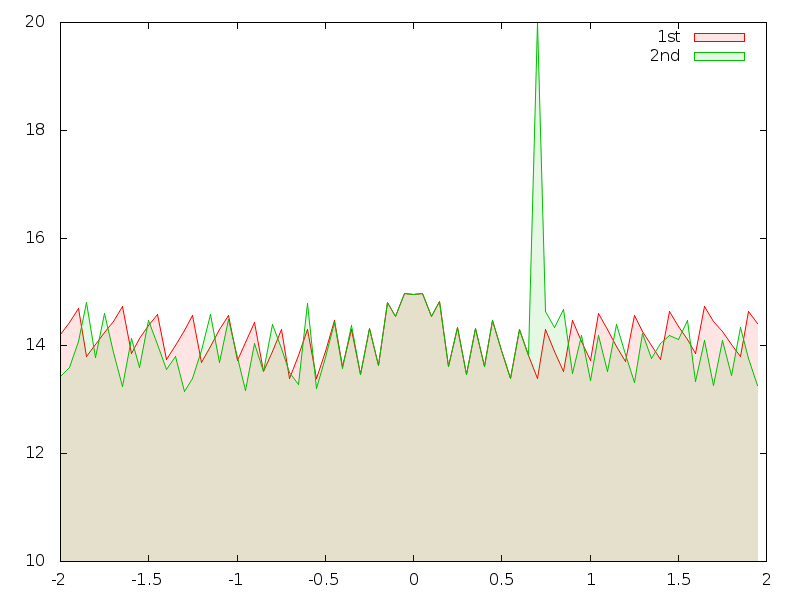
\includegraphics[height=0.25\textheight]{/home/luki/Documents/Numerki/Pracownia/graphs.png} %:)
        \captionof{figure}{Dokładność metod testowanych dla małych liczb}
        \label{fig:graphs}
    \end{minipage}
    \begin{minipage}[c]{0.5\linewidth}
        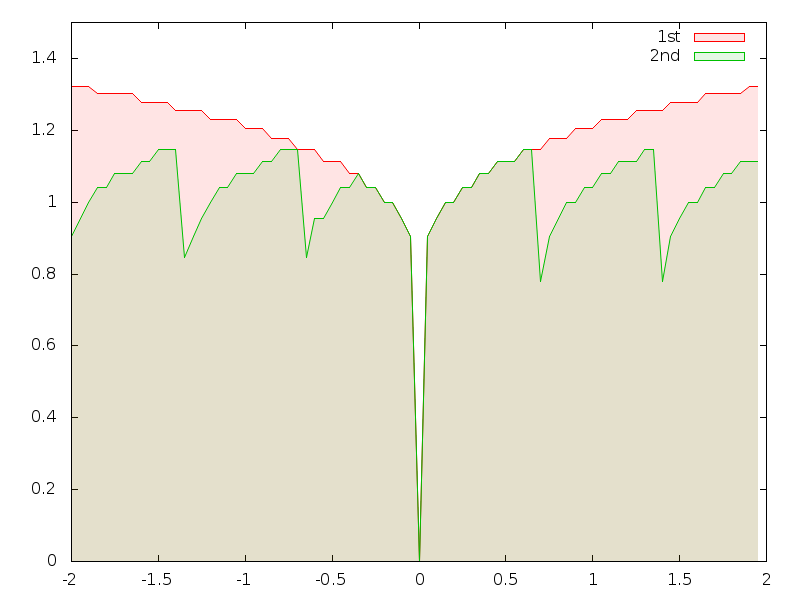
\includegraphics[height=0.25\textheight]{/home/luki/Documents/Numerki/Pracownia/numbs.png}
        \captionof{figure}{Ilość iteracji dla małych liczb}
        \label{fig:numbs}
    \end{minipage}
\end{figure}
\begin{figure}[h]
    \begin{minipage}[c]{0.5\linewidth}
        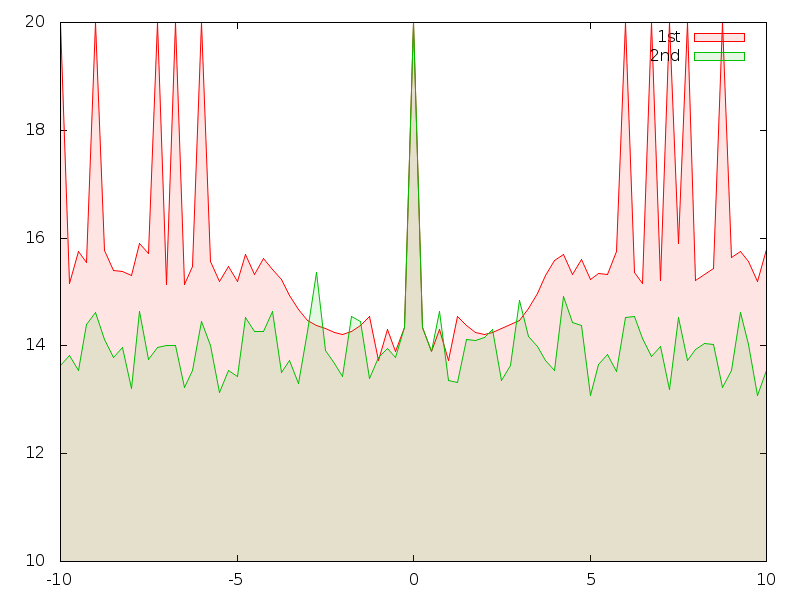
\includegraphics[height=0.25\textheight]{/home/luki/Documents/Numerki/Pracownia/graphm.png}
        \captionof{figure}{Dokładność metod testowanych dla średnich liczb}
        \label{fig:graphm}
    \end{minipage}
    \begin{minipage}[c]{0.5\linewidth}
        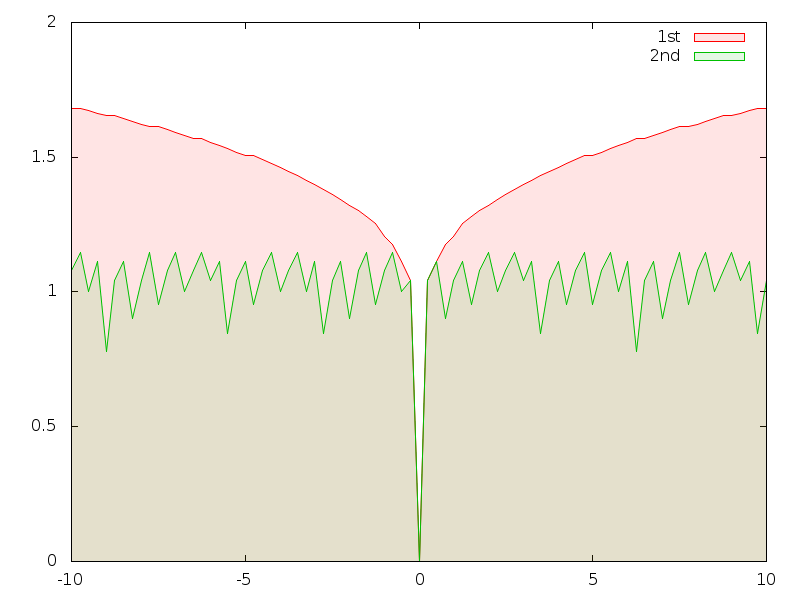
\includegraphics[height=0.25\textheight]{/home/luki/Documents/Numerki/Pracownia/numbm.png}
        \captionof{figure}{Ilość iteracji dla średnich liczb}
        \label{fig:numbm}
    \end{minipage}
\end{figure}
\begin{figure}[h]
    \begin{minipage}[c]{0.5\linewidth}
        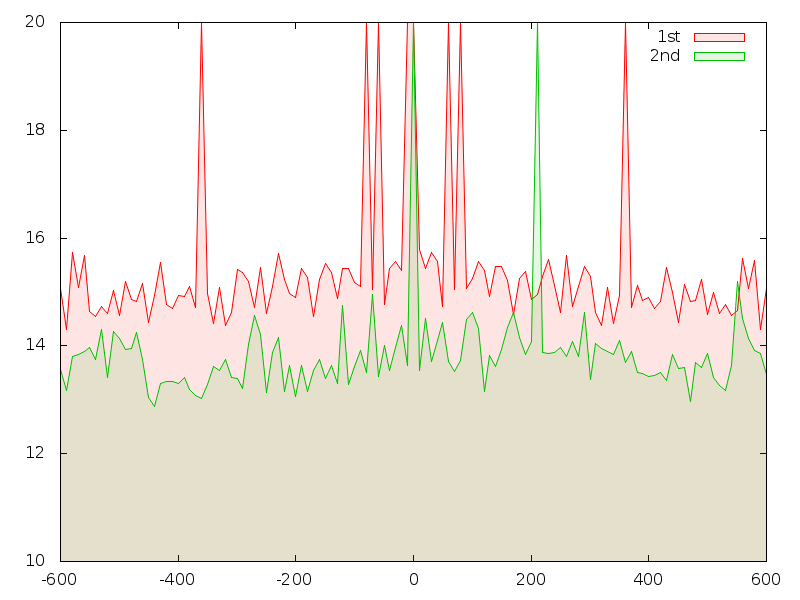
\includegraphics[height=0.25\textheight]{/home/luki/Documents/Numerki/Pracownia/graphb.png}
        \captionof{figure}{Dokładność metod testowanych dla dużych liczb}
        \label{fig:graphb}
    \end{minipage}
    \begin{minipage}[c]{0.45\linewidth}
        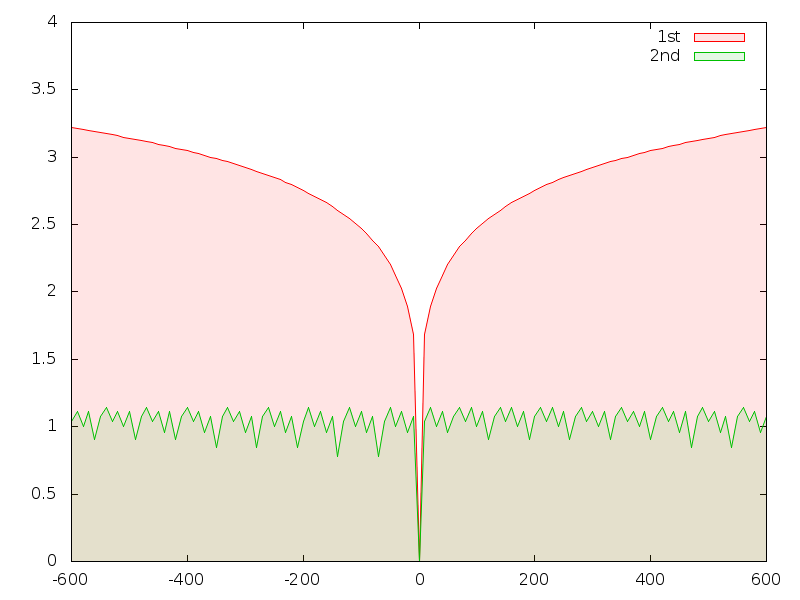
\includegraphics[height=0.25\textheight]{/home/luki/Documents/Numerki/Pracownia/numbb.png}
        \captionof{figure}{Ilość iteracji dla dużych liczb}
        \label{fig:numbb}
    \end{minipage}
\end{figure}
\subsection{Obserwacje}
Jak zostało wcześniej wspomniane, zakładamy ze metoda $exp$ (jako wbudowana) zwraca wynik z błędem na poziomie błędu arytmetyki. Dzięki temu dokładność pozostałych metod można oszacować przez porównanie ich wyników z wynikiem $exp$.
Wykresy~\ref{fig:graphs} i \ref{fig:numbs} nie oferują żadnych zaskakujących obserwacji. Całkowicie zgadzają się one z wnioskami wyciągniętymi z analizy wzorów. Metoda $\Psi$ wydaje się lepsza od $\Phi$ zarówno pod względem błędu jak i ilości iteracji.
Obserwacje z wykresów~\ref{fig:graphm} i \ref{fig:numbm} powoli przestają przystawać do przewidywań. O ile faktycznie ilość iteracji wykonywanych przez $\Psi$ jest mniejsza od $\Phi$, to porównanie błędów jest korzystne dla $\Phi$, zupełnie inaczej niż wynikało z analizy.
Wykresy~\ref{fig:graphb} i \ref{fig:numbb} potwierdzają "dziwną" obserwacje: metoda $\Psi$ liczy $e^x$ z większym błędem niz $\Phi$. Zyskuje jednak na wymaganej ilości iteracji: wykonuje ich nawet 100x mniej.
\subsection{Podsumowanie}
Wniosek jest oczywisty: metoda $\Psi$ poświecą cześć dokładności metody $\Phi$ na rzecz o wiele krótszego czasu wykonania. Czemu jednak tak się dzieje? Aby to wytłumaczyć, należy cofnąć się do analizy błędów, która wykonaliśmy przed rozpoczęciem obliczeń (\ref{sec:bl}). Zauważyliśmy tam, ze nie bierzemy pod uwagę błędu obliczania $m$ i $u$, a przyjmujemy je za dane. Przyjrzyjmy się wiec dokładnie, jak są liczone. Używa się w tym celu wielkości pomocniczych:
\begin{gather}
  z := \frac{x}{\ln 2}\\
  m := \lfloor z + sgn(x)\frac{1}{2} \rfloor\\
  w := z - m\\
  u := w\ln 2\\
\end{gather}
Zauważmy, ze  $|z - m| < \frac{1}{2}$. W szczególności: gdy $z\rightarrow m$, to $w$ (a co za tym idzie $u$) może być obliczone z dużym błędem. Tak wiec końcowy wynik, $2^m*\Phi(u)$ może być obarczone błędem powstającym właśnie przez odejmowanie bliskich sobie liczb.
\indent Takie porównanie pozostawia jednak kilka pytań. Czy  ilość iteracji wykonywanych przez metody ma tak duże znaczenie, by strata kilku miejsc zerowych dokładności przez metodę $\Psi$ w porównaniu do $\Phi$ dawała widoczne korzyści? Jak w porównaniu do nich wypada funkcja wbudowana $exp$? Jak mogla ona zostać zaimplementowana?
\section{Czas obliczeń}
\subsection{Porównanie}
Aby odpowiedzieć na powstałe pytania, porównałem faktyczny czas upływający od wywołania metody do otrzymania wyniku. Przedstawię tutaj wynikające z tego wnioski.\\
\begin{minipage}[c]{0.45\linewidth}
    \begin{tabular}{|l|l|l|l|}
        \hline
        $n$ & $T(\Phi, n)$ & $T(\Psi, n)$ & $T(exp, n)$\\
        \hline
        -562.23 & 131747 & 8480  & 145 \\
         -413.1 & 105884 & 7881  & 150 \\
        -119.78 & 47158 & 14338 & 156 \\
        -104.42 & 70746  & 32075 & 160 \\
         -89.31 & 50313  & 16304 & 163 \\
         -14.58 & 21303  & 12849 & 157 \\
           2.29 & 12340  & 12241 & 160 \\
          18.73 & 18104  & 13845 & 166 \\
          34.21 & 22619  & 14636 & 154 \\
          80.37 & 37677  & 13666 & 155 \\
         287.81 & 73165  & 11215 & 167 \\
         473.95 & 112880 & 12216 & 249 \\
          592.5 & 138690 & 11868 & 161 \\
        \hline
    \end{tabular}
    \captionof{table}{Wybrane przykłady z Tabeli \ref{tab:Tn} \\{\small{(zawartej w dodatku \ref{sec:appendix})}}\\{\tiny{Tabela \ref{tab:oznaczenia} objaśnia oznaczenia}}}
    \label{tab:przyklady}
\end{minipage}
\begin{minipage}[c]{0.45\linewidth}
        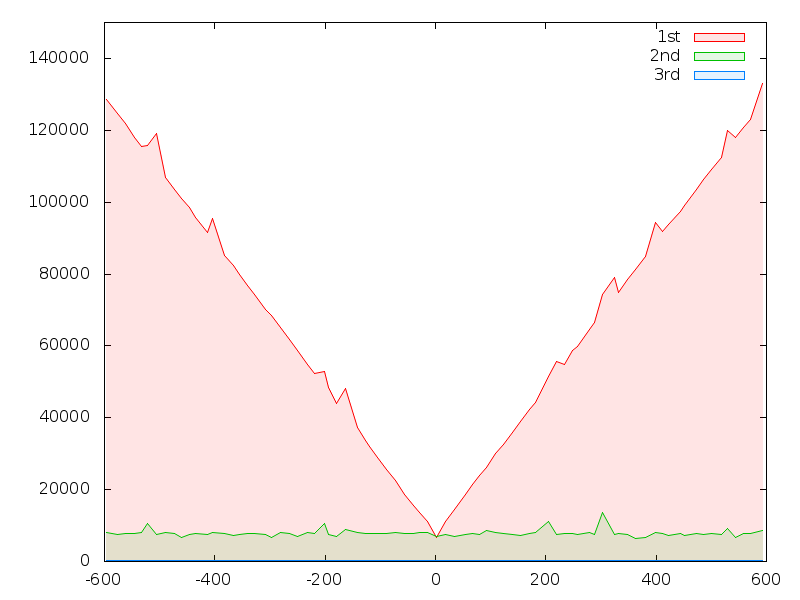
\includegraphics[scale=0.3]{/home/luki/Documents/Numerki/Pracownia/czas.png}
        \captionof{figure}{Czas obliczania funkcji - wykres}
        \label{fig:czas}
\end{minipage}
\subsection{Legenda}
Wyniki w tabeli~\ref{tab:przyklady} zostały podane w milisekundach i przedstawiają czas obliczeń 1000 wywołań odpowiednich funkcji. Porównanie to zostało wykonane na komputerze dysponującym 1GB RAM i procesorem 1,6GHz. Oznaczenia przyjęte na wykresie~\ref{fig:czas}:
\begin{table}[h]
\centering
\begin{tabular}{r c l}
  \hline
  Oznaczenie & Kolor linii & Metoda\\
  \hline
  1st        & Czerwony    & $\Phi$\\
  2nd        & Zielony     & $\Psi$\\
  3rd        & Niebieski   & $exp$\\
  \hline
\end{tabular}
\label{tab:legendawykr2}
\caption{Legenda do wykresu \ref{fig:czas}}
\end{table}
\subsection{Komentarze}
Obserwacje z tabeli~\ref{tab:przyklady} potwierdzają, ze ilość wykonywanych iteracji ma znaczący wpływ na czas obliczeń. Co więcej, metoda $\Phi$ była widocznie wolniejsza od metody $\Psi$. Oznacza to, ze używanej metody obliczania $e^x$ trzeba by dobierać do konkretnego zastosowania: gdy zależy nam na prędkości (np przy liczeniu nietrywialnej funkcji wymagającej wielokrotnego policzenia $e^x$) lepiej byłoby użyć metody $\Psi$, jednak oznaczałoby to stratę dokładności. Gdy zależałoby na dokładności, lepsza okazałaby się metoda $\Phi$. Jednak z tabeli wynika coś jeszcze: metoda $exp$ bije obie metody zaimplementowane dla celów tej pracowni zarówno pod względem prędkości (i to znacząco, dla dowolnego argumentu była 100x szybsza), jak i dokładności (bo założyliśmy, ze zwraca wyniki na poziomie błędu arytmetyki). Co ciekawe, funkcja ta wydaje się mieć prawie stały czas działania (nie rośnie on dla argumentów dalszych od 0, podobnie jak $\Psi$). Należałoby jednak upewnić się jeszcze, czy na pewno metoda $exp$ jest tak dokładna, jak zakładamy. Jest to trudne, gdyż wymagałoby porównania z zewnętrznym źródłem (np z wynikami zwracanymi przez serwis Wolfram Alpha), bo nie wiadomo, czy $exp$ nie jest zaimplementowano bezpośrednio na komendach procesora i wobec tego wspólna dla wielu jeżyków programowania. Można by też użyć systemu typu Maple wykonującego obliczenia symbolicznie, jednak jest to praktycznie temat na osobną pracownię.
\section{Zakończenie}
\subsection{Ogólne podsumowanie metod}
Głównym wnioskiem płynącym z porównania metod $\Phi$ i $\Psi$ jest stwierdzenie, że obie należy stosować w rożnych przypadkach. $\Phi$ - gdy zależy na dokładności, a $\Psi$ - na szybkości. Jednak obie są o wiele gorsze od $exp$, wiec albo opiera się ona na zupełnie innym pomyśle, albo omija narzut spowodowany przez język programowania i jest bezpośrednio zaimplementowana w komendach procesora. Najprawdopodobniej mamy do czynienia z połączeniem obu tych podejść. Niestety weryfikacja tego jest trudna, gdyż nie udało się dotrzeć do miejsca w którym $exp$ jest bezpośrednio zaimplementowana w bibliotece $<cmath>$, gdyż każde definicja funkcji odwołuje się do kolejnej (zwykle ukrytej w innej bibliotece lub wbudowanej), bez praktycznie jakichkolwiek przekształceń.
\subsection{Inne pomysły}
Prowadzi to do rozważań: jak inaczej można obliczać funkcję $e^x$? Jednym z podejść mogłoby być ulepszenie funkcji $\Psi$ przez stablicowanie dość gęsto wartości $e^x$ obliczonych z dużą dokładnością dla argumentów $[-\frac{\ln 2}{2}, \frac{\ln 2}{2}]$, a następnie liczenie $m$ w sposób pozwalający uniknąć utraty cyfr dokładnych. Innym przybliżenie $e^x$ przez pewien wielomian (w zakresie arytmetyki 64-bitowej) i liczenie jego wartości.
\newpage
\thispagestyle{empty}
\appendix
\section{Pełna tabela porównań czasów obliczania $e^x$ przez omawiane funkcje}
\label{sec:appendix}
    \begin{longtable}{|l|l|l|l|}
        \hline
        $n$ & $T(\Phi, n)$ & $T(\Psi, n)$ & $T(exp, n)$\\
        \hline
        \endhead
        \hline
        \endfoot
        -596.17 & 148180 & 12506 & 200 \\
        -576.14 & 137177 & 10745 & 158 \\
        -562.23 & 131747 & 8480 & 145 \\
        -545.85 & 133589 & 9229 & 145 \\
        -532.07 & 142841 & 10216 & 146 \\
        -521.65 & 124822 & 7451 & 146 \\
        -506.14 & 122918 & 7014 & 145 \\
        -490.08 & 118993 & 8238 & 146 \\
        -473.51 & 115704 & 8036 & 145 \\
        -460.79 & 113860 & 6908 & 146 \\
        -446.38 & 115571 & 8103 & 146 \\
        -434.73 & 107977 & 8089 & 148 \\
         -413.1 & 105884 & 7881 & 150 \\
        -404.41 & 98907 & 7851 & 146 \\
        -382.37 & 96263 & 9228 & 146 \\
        -365.74 & 89563 & 7296 & 146 \\
         -354.6 & 89970 & 10837 & 162 \\
        -340.74 & 87522 & 7464 & 145 \\
        -328.28 & 83809 & 8646 & 177 \\
        -307.64 & 78310 & 7969 & 146 \\
        -297.89 & 81706 & 7212 & 145 \\
        -281.32 & 74355 & 7701 & 379 \\
        -264.33 & 75064 & 12189 & 167 \\
        -250.71 & 67190 & 7114 & 180 \\
        -232.18 & 64807 & 11163 & 146 \\
         -219.7 & 56287 & 8170 & 153 \\
        -201.38 & 58624 & 7854 & 146 \\
        -193.77 & 51570 & 9015 & 158 \\
        -179.33 & 52793 & 9110 & 147 \\
        -163.65 & 52109 & 13024 & 165 \\
        -140.71 & 58414 & 12993 & 162 \\
        -126.98 & 49596 & 12846 & 168 \\
        -119.78 & 47158 & 14338 & 156 \\
        -104.42 & 70746 & 32075 & 160 \\
         -89.31 & 50313 & 16304 & 163 \\
         -73.33 & 46463 & 13700 & 159 \\
         -56.07 & 39545 & 16506 & 162 \\
         -40.44 & 28807 & 16155 & 162 \\
         -29.89 & 26124 & 21917 & 162 \\
         -14.58 & 21303 & 12849 & 157 \\
           2.29 & 12340 & 12241 & 160 \\
          18.73 & 18104 & 13845 & 166 \\
          34.21 & 22619 & 14636 & 154 \\
          54.19 & 29470 & 16317 & 173 \\
          67.84 & 39643 & 15080 & 165 \\
          80.37 & 37677 & 13666 & 155 \\
          91.98 & 39696 & 13499 & 159 \\
         108.24 & 48243 & 15110 & 159 \\
         123.15 & 46979 & 14359 & 158 \\
          138.7 & 51271 & 13978 & 160 \\
         154.13 & 56626 & 13351 & 155 \\
         170.26 & 60691 & 14501 & 155 \\
         180.91 & 61728 & 14751 & 157 \\
          204.8 & 78896 & 16940 & 159 \\
         219.56 & 82391 & 16479 & 162 \\
         233.73 & 76855 & 8102 & 146 \\
         248.62 & 67957 & 7550 & 145 \\
          256.7 & 63042 & 11322 & 155 \\
         279.96 & 72897 & 10338 & 146 \\
         287.81 & 73165 & 11215 & 167 \\
         303.05 & 77112 & 11944 & 146 \\
         324.25 & 79607 & 7197 & 154 \\
         330.84 & 83817 & 7186 & 157 \\
         348.27 & 85332 & 7936 & 146 \\
         363.36 & 88990 & 10888 & 165 \\
         380.05 & 98772 & 9236 & 159 \\
         398.46 & 99692 & 7561 & 145 \\
         412.29 & 100074 & 10498 & 146 \\
         423.13 & 102765 & 7733 & 155 \\
         443.57 & 103733 & 8243 & 167 \\
         451.24 & 110008 & 8520 & 146 \\
         473.95 & 112880 & 12216 & 249 \\
         485.82 & 115843 & 9207 & 157 \\
         500.45 & 117960 & 12699 & 155 \\
         518.14 & 129029 & 9128 & 145 \\
         528.67 & 125099 & 7433 & 151 \\
         544.34 & 132195 & 6737 & 147 \\
         558.64 & 130792 & 8351 & 145 \\
         570.43 & 131566 & 8301 & 167 \\
          592.5 & 138690 & 11868 & 161 \\
        \hline       
    \caption{Czas obliczeń dla funkcji testowanych i wbudowanej\\ {\small{Tabela \ref{tab:oznaczenia} zawiera oznaczenia.}}}
    \label{tab:Tn}
    \end{longtable}
\end{document}

